\documentclass[a4paper]{article}
\usepackage{times}
\usepackage[utf8]{inputenc}
\usepackage{selinput}
\usepackage{upquote}
\usepackage[margin=2cm, rmargin=4cm, tmargin=3cm]{geometry}
\usepackage{tcolorbox}
\usepackage{xspace}
\usepackage[french]{babel}
\usepackage{url}
\usepackage{hyperref}
\usepackage{fontawesome5}
\usepackage{marginnote}
\usepackage{ulem}
\usepackage{tcolorbox}
\usepackage{graphicx}
%\usepackage[top=Bcm, bottom=Hcm, outer=Ccm, inner=Acm, heightrounded, marginparwidth=Ecm, marginparsep=Dcm]{geometry}


\newtcolorbox{Example}[1]{colback=white,left=20pt,colframe=slideblue,fonttitle=\bfseries,title=#1}
\newtcolorbox{Solutions}[1]{colback=white,left=20pt,colframe=green,fonttitle=\bfseries,title=#1}
\newtcolorbox{Conseils}[1]{colback=white,left=20pt,colframe=slideblue,fonttitle=\bfseries,title=#1}
\newtcolorbox{Warning}[1]{colback=white,left=20pt,colframe=warning,fonttitle=\bfseries,title=#1}

\setlength\parindent{0pt}

  %Exercice environment
  \newcounter{exercice}
  \newenvironment{Exercice}[1][]
  {
  \par
  \stepcounter{exercice}\textbf{Question \arabic{exercice}:} (\faClock \enskip \textit{#1})
  }
  {\bigskip}
  

% Title
\newcommand{\titre}{\begin{center}
  \section*{Algorithmes et Pensée Computationnelle}
\end{center}}
\newcommand{\cours}[1]
{\begin{center} 
  \textit{#1}\\
\end{center}
  }


\newcommand{\exemple}[1]{\newline~\textbf{Exemple :} #1}
%\newcommand{\attention}[1]{\newline\faExclamationTriangle~\textbf{Attention :} #1}

% Documentation url (escape \# in the TP document)
\newcommand{\documentation}[1]{\faBookOpen~Documentation : \href{#1}{#1}}

% Clef API
\newcommand{\apikey}[1]{\faKey~Clé API : \lstinline{#1}}
\newcommand{\apiendpoint}[1]{\faGlobe~Url de base de l'API \href{#1}{#1}}

%Listing Python style
\usepackage{color}
\definecolor{slideblue}{RGB}{33,131,189}
\definecolor{green}{RGB}{0,190,100}
\definecolor{blue}{RGB}{121,142,213}
\definecolor{grey}{RGB}{120,120,120}
\definecolor{warning}{RGB}{235,186,1}

\usepackage{listings}
\lstdefinelanguage{texte}{
    keywordstyle=\color{black},
    numbers=none,
    frame=none,
    literate=
           {é}{{\'e}}1
           {è}{{\`e}}1
           {ê}{{\^e}}1
           {à}{{\`a}}1
           {â}{{\^a}}1
           {ù}{{\`u}}1
           {ü}{{\"u}}1
           {î}{{\^i}}1
           {ï}{{\"i}}1
           {ë}{{\"e}}1
           {Ç}{{\,C}}1
           {ç}{{\,c}}1,
    columns=fullflexible,keepspaces,
	breaklines=true,
	breakatwhitespace=true,
}
\lstset{
    language=Python,
	basicstyle=\bfseries\footnotesize,
	breaklines=true,
	breakatwhitespace=true,
	commentstyle=\color{grey},
	stringstyle=\color{slideblue},
  keywordstyle=\color{slideblue},
	morekeywords={with, as, True, False, Float, join, None, main, argparse, self, sort, __eq__, __add__, __ne__, __radd__, __del__, __ge__, __gt__, split, os, endswith, is_file, scandir, @classmethod},
	deletekeywords={id},
	showspaces=false,
	showstringspaces=false,
	columns=fullflexible,keepspaces,
	literate=
           {é}{{\'e}}1
           {è}{{\`e}}1
           {ê}{{\^e}}1
           {à}{{\`a}}1
           {â}{{\^a}}1
           {ù}{{\`u}}1
           {ü}{{\"u}}1
           {î}{{\^i}}1
           {ï}{{\"i}}1
           {ë}{{\"e}}1
           {Ç}{{\,C}}1
           {ç}{{\,c}}1,
    numbers=left,
}

\newtcbox{\mybox}{nobeforeafter,colframe=white,colback=slideblue,boxrule=0.5pt,arc=1.5pt, boxsep=0pt,left=2pt,right=2pt,top=2pt,bottom=2pt,tcbox raise base}
\newcommand{\projet}{\mybox{\textcolor{white}{\small projet}}\xspace}
\newcommand{\optionnel}{\mybox{\textcolor{white}{\small Optionnel}}\xspace}
\newcommand{\advanced}{\mybox{\textcolor{white}{\small Pour aller plus loin}}\xspace}
\newcommand{\auto}{\mybox{\textcolor{white}{\small Auto-évaluation}}\xspace}


\usepackage{environ}
\newif\ifShowSolution
\NewEnviron{solution}{
  \ifShowSolution
	\begin{Solutions}{\faTerminal \enskip Solution}
		\BODY
	\end{Solutions}
  \fi}


  \usepackage{environ}
  \newif\ifShowConseil
  \NewEnviron{conseil}{
    \ifShowConseil
    \begin{Conseils}{\faLightbulb \quad Conseil}
      \BODY
    \end{Conseils}

    \fi}

    \usepackage{environ}
  \newif\ifShowWarning
  \NewEnviron{attention}{
    \ifShowWarning
    \begin{Warning}{\faExclamationTriangle \quad Attention}
      \BODY
    \end{Warning}

    \fi}
  

%\newcommand{\Conseil}[1]{\ifShowIndice\ \newline\faLightbulb[regular]~#1\fi}



\usepackage{listings}
\usepackage{array}
\newcolumntype{C}[1]{>{\centering\let\newline\\\arraybackslash\hspace{0pt}}m{#1}}

\begin{document}

% Change the following values to true to show the solutions or/and the hints
\ShowSolutionfalse
\ShowConseiltrue
\titre
\cours{Programmation de base}

Le but de cette séance est d'aborder des notions de base en programmation. Au terme de cette séance, l'étudiant sera capable de: \\

\begin{itemize}
    \item Comprendre les différentes représentations de nombres.
	\item Définir des variables et comprendre les types de variables existants.
	\item Utiliser des notions d'algèbre booléenne.
    \item Ecrire des branchements conditionnels.\\
\end{itemize} 

Les langages qui seront utilisés pour cette séance sont Java et Python. Assurez-vous d'avoir bien installé Intellij. Si vous rencontrez des difficultés, n'hésitez pas à vous référer au guide suivant: \href{https://moodle.unil.ch/mod/resource/view.php?id=1761727}{tutoriel d'installation des outils et prise en main de l'environnement de travail}.\\

\section{Représentation de nombres entiers}

\begin{Exercice}[5 minutes] \textbf{Entiers non signés}\\
	Sur 8 bits, convertir 113$_{(10)}$ en base binaire.
   
    \begin{conseil}
		Faire un tableau comme présenté dans la diapositive 10 du cours (programmation de base). Essayer de décomposer le nombre en une somme de puissances de 2.
    \end{conseil}
    
    \begin{solution}
        Méthode 1: Utiliser la division par 2 comme vu dans la première séance d'exercices\\
        
        Méthode 2 : Utiliser les puissances de 2 pour décomposer le nombre (vu également dans la première séance d'exercices).
        
        113 = 64 + 32 + 16 + 1 = 1 * $2^6$ + 1 * $2^5$ + 1* $2^4$ + 1 * $2^0$ \\
        
        \begin{tabular}{| p{1cm} | p{1cm} | p{1cm} | p{1cm} | p{1cm} | p{1cm} | p{1cm} | p{1cm} | p{1cm} |} 
            \hline
	      	$2^7$ & $2^6$ & $2^5$ & $2^4$ & $2^3$ & $2^2$ & $2^1$ & $2^0$ \\ [0.5ex]
	    	\hline
            128 & 64 & 32 & 16 & 8 & 4 & 2 & 1 \\ [0.5ex] 
            \hline
            0 & 1 & 1 & 1 & 0 & 0 & 0 & 1 \\ [0.5ex] 
            \hline
        \end{tabular} \\
        
        On obtient donc 01110001$_{(2)}$ \\
    \end{solution}
\end{Exercice}

\begin{Exercice}[5 minutes] \textbf{Entiers signés négatifs}\\
    En utilisant le résultat de la question précédente, convertir sur 8 bits -113$_{(10)}$ en base binaire. \\

    \begin{conseil}
        \begin{itemize}
        	\item Il faut prendre la représentation sur 7 bits d'un nombre entier non signé.
        	\item On rajoute un 8ème bit qui sera le signe.
        	\item Pour cet exercice, reprendre l'expression non signée de la question précédente (question 1 - Entiers non signés) et changer le premier bit en conséquence.
        	\item Le premier bit vaut 0 pour un nombre positif et 1 pour un nombre négatif.
        \end{itemize} 
    \end{conseil}
    
    \begin{solution}
         113$_{(10)}$ = 01110001$_{(2)}$ \\
         
         En changeant le premier bit à 1 pour faire passer le nombre en nombre négatif on obtient : \\
         
         -113$_{(10)}$ = 11110001$_{(2)}$ \\
    \end{solution}
\end{Exercice}

\begin{Exercice}[5 minutes] \textbf{Complément à 1}\\
    Écrire le complément à 1 de -113$_{(10)}$ . \\

	Quelle est la différence entre cette méthode et la précédente ?

    \begin{conseil}
        \begin{itemize}
        	\item L'opposé de 0 en binaire est 1 et inversément.
        	\item Pour étudier la différence, il faut regarder les différentes manières d'exprimer -0 en binaire (se référer à la diapositive 11 du cours de la semaine 3).
        \end{itemize} 
    \end{conseil}
    
    \begin{solution}
    	113$_{(10)}$ = 01110001$_{(2)}$ \\
    	
        \begin{tabular}{| p{1cm} | p{1cm} | p{1cm} | p{1cm} | p{1cm} | p{1cm} | p{1cm} | p{1cm} | p{1cm} |} 
            \hline
            0 & 1 & 1 & 1 & 0 & 0 & 0 & 1 \\ [0.5ex] 
            \hline
            not & not & not & not & not & not & not & not \\ [0.5ex]
            \hline
            1 & 0 & 0 & 0 & 1 & 1 & 1 & 0 \\ [0.5ex]
            \hline
        \end{tabular} \\
        
        avec cette méthode, -113$_{(10)}$ = 10001110$_{(2)}$ \\
        
        L'intervalle de cette méthode ne change pas par rapport à la précédente. Par contre, l'expression de -0 sera différente.\\
        
        Signé: -0$_{(10)}$ = 10000000$_{(2)}$ \\
        
        Complément à 1: -0$_{(10)}$ = 11111111$_{(2)}$ \\
        
        Les deux ont le même intervalle: [-127$_{(10)}$,+127$_{(10)}$] \\
        
    \end{solution}
\end{Exercice}

\begin{Exercice}[5 minutes] \textbf{Complément à 2}\\
    Quel est le complément à 2 de -113$_{(10)}$ et quelle est l'utilité de cette représentation ? \\

    \begin{conseil}
    
    Exemple du cours avec 87$_{(10)}$ \\
    
    87$_{(10)}$ = 01010111$_{(2)}$ \\
    
         \begin{tabular}{| p{1cm} | p{1cm} | p{1cm} | p{1cm} | p{1cm} | p{1cm} | p{1cm} | p{1cm} | p{1cm} |} 
            \hline
            a & 0 & 1 & 0 & 1 & 0 & 1 & 1 & 1 \\ [0.5ex] 
            \hline
            b & 1 & 0 & 1 & 0 & 1 & 0 & 0 & 0 \\ [0.5ex]
            \hline
            c & 1 & 0 & 1 & 0 & 1 & 0 & 0 & 1 \\ [0.5ex]
            \hline
        \end{tabular} \\
        
        a : convertir le nombre en binaire \\
        
        b : inverser tous les bits \\
        
        c : rajouter 1 au nombre pour obtenir le complément à 2 \\
        
        On obtient donc -87$_{(10)}$ = 10101001$_{(2)}$ \\
    \end{conseil}
    
    \begin{solution}
    	Ici, il suffit donc d'ajouter 1 au complément à 1 de -113$_{(10)}$ \\
    	
    	On obtient donc 10001111$_{(2)}$ \\
    	
    	Concernant l'intervalle, il est changé, étant donné qu'il n'existe plus qu'une seule représentation possible pour -0$_{(10)}$. \\
    	
    	Le nouvel intervalle est donc [-128$_{(10)}$,+127$_{(10)}$]
        
    \end{solution}
\end{Exercice}

\begin{Exercice}[10 minutes] \textbf{Floating point}\\
    
    Voici la représentation en binaire d'un nombre à virgule flottante: \\
    
     \begin{tabular}{| p{1cm} | p{3cm} | p{9.5cm} | p{1cm} | p{1cm} | p{1cm} | p{1cm} | p{1cm} | p{1cm} |} 
            \hline
            signe & exposant & mantisse \\ [0.5ex] 
            \hline
            0 & 10110101 & 01000001000000000000001 \\ [0.5ex]
            \hline
	\end{tabular}
	\\
    Que vaut cette représentation en base 10 ? Utiliser la représentation des floating points (avec un biais de 127). Arrondir les résultats intermédiaires et la valeur finale au 3ème chiffre significatif après la virgule. \\
	
    \begin{conseil}
    
    \begin{itemize}
    	\item Se référer à la diapositive 15 du cours (programmation de base) pour plus de détails.
    	\item Poser chaque calcul, et ensuite tout fusionner avec la formule.
    	\item L'exposant et la mantisse sont des entiers positifs, donc non signés.
    	\item Pour vérifier votre résultat, vous pouvez utiliser l'outil suivant: \url{https://www.h-schmidt.net/FloatConverter/IEEE754.html}
    \end{itemize}
    
    \end{conseil}
    
    \begin{solution}
        \begin{itemize}
        	\item Signe du nombre : $(-1)^{signe}$ = $(-1)^0$ = 1
        	\item Exposant en base 10 : 10110101$_{(2)}$ = 181$_{(10)}$
        	\item Pour obtenir l'exposant, il faut encore lui appliquer le biais, il faut soustraire 127 à notre résultat. Ici on aura $2^{(181-127)}$ = $2^{54}$
        	\item Mantisse : 01000001000000000000001$_{(2)}$ = 1 + 1*$2^{-2}$ + 1*$2^{-8}$ + 1*$2^{-23}$ = 1.254$_{(10)}$
        	\item Valeur = Signe * Mantisse * $2^{exposant-127}$ = 1 * 1.254 * $2^{54}$ = 2.259 * $10^{16}$
        \end{itemize}
    \end{solution}
\end{Exercice}
\newpage

\newpage

\section{Typage}

Le but de cette partie des travaux pratiques est de comprendre les notions de typage statique et dynamique, ainsi que leur impact sur l’exécution et la gestion des erreurs. \\

\begin{Exercice}[5 minutes]  \textbf{Les types de variables}\\
    
    Quelles sont les principaux types de variables (donnez en 3), comment les déclareriez-vous en Python et en Java ? \\

    \begin{conseil}
    
        Se référer aux diapositives du cours ou à la documentation officielle des langages de programmation.
        
    \end{conseil}
    \begin{solution}
    
        Les principaux types de variables sont les suivants : \lstinline{Integer (int), Float, String (str), Boolean (bool)}.\\

		En Python :    
        
    	\lstinputlisting{updated/solutions/Question6.py} 
    	
    	
    	En Java : 
    	
    	\lstinputlisting{updated/solutions/Question6.java} 
    	
    	Il existe d'autres types de variable, comme par exemple les \lstinline{double}.
 
    \end{solution}
\end{Exercice}


\begin{Exercice}[10 minutes]  \textbf{Typage statique et dynamique}\\
    
    Parmi ces différents programmes, lesquels pourront être exécutés sans problème et lesquels lèveront des erreurs? Dans le cas où ils génèreraient des erreurs, expliquez la raison de ces erreurs.\\
    
    \textbf{Java :}
    
    \lstinputlisting{updated/Questions/Question7.java} 
    
    \textbf{Python :}
    
    \lstinputlisting{updated/Questions/Question7.py} 
    

    \begin{conseil}
    
        En Java, le type est statique, ce qui signifie qu'à partir du moment où vous créez une variable, un type va lui être attribué (par vous ou par le code en lui-même par déduction). Ce type ne pourra pas être changé, et si vous tentez de le faire (en lui attribuant une valeur d'un autre type par exemple), une erreur sera levée. \\

En Python, le typage est dynamique, il est donc tout à fait possible de changer le type d'une variable sans déclencher d'erreur. \\

    \end{conseil}

    \begin{Example}{\faExclamationTriangle \quad Erreurs fréquentes}
        Au cas où vous exécuteriez les programmes 2, 4 et 5 et rencontriez l'erreur suivante: \lstinline{Exception in thread "main" java.lang.UnsupportedClassVersionError: ... has been compiled by a more recent version of the Java Runtime (class file version 54.0), this version of the Java Runtime only recognizes class file versions up to 52.0}, suivez les étapes ci-dessous:
        \begin{enumerate}
            \item Mettez à jour votre JDK en téléchargeant la version adéquate via le lien suivant: \url{https://www.oracle.com/java/technologies/downloads/}.
            \item Une fois votre JDK installé, redémarrez IntelliJ
            \item Dans la barre de menus, cliquez sur \textbf{Run $>$ Edit Configurations}.
            \item Dans la fenêtre qui apparaitra (capture ci-dessous), sélectionnez la version du JRE la plus récente.
        \end{enumerate}
        
    \end{Example}
    \begin{figure}[h]
        \centering
        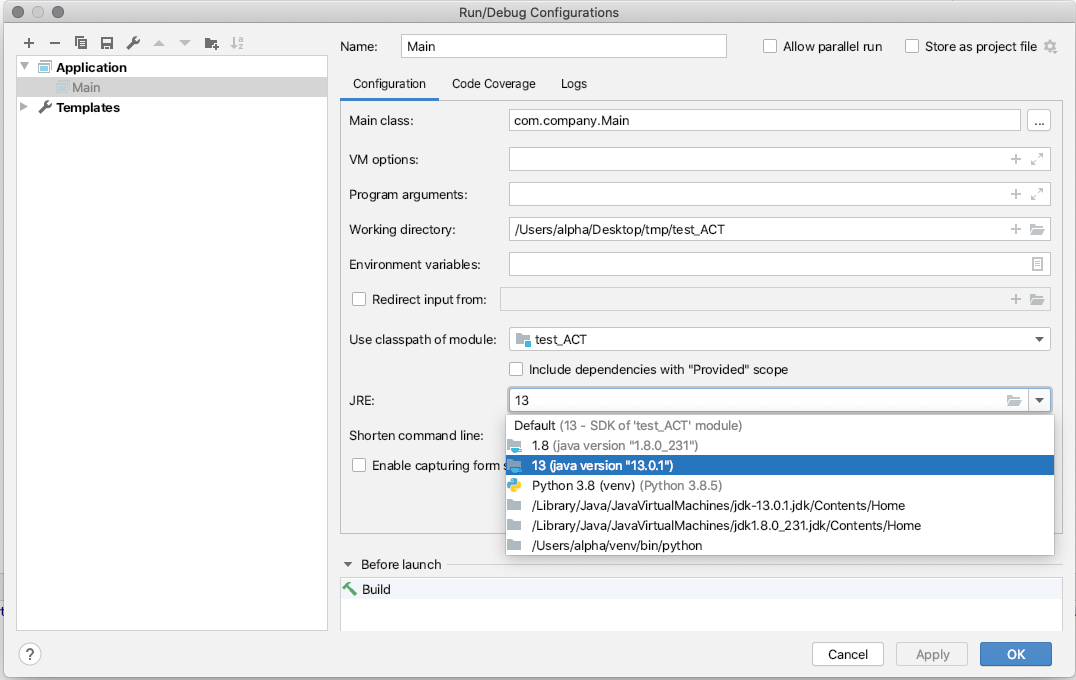
\includegraphics[width=1\textwidth]{resources/jre.png}
        \caption{Fenêtre de configuration de l'environnement de développement Java.}
    \end{figure}
    \begin{solution}

        \textbf{En Java}        
        \begin{itemize}
        	\item Programme 1 : OK
        	\item Programme 2 : Ce code ne fonctionnera pas car on essaye de changer le type de la variable\_2, ce qui est impossible avec un typage statique comme en java. Ici le type de la variable est ``déduit'' lors de l'exécution du programme.
        	\item Programme 3 : Tout comme le programme précédent, ce code ne fonctionnera pas car on essaye de changer le type de la variable\_2, ce qui est impossible avec un typage statique comme en java.
        	\item Programme 4 : Ce code ne fonctionnera pas car on essaye de changer le type de la variable\_1, ce qui est impossible avec un typage statique comme en java. Ici le type de la variable est ``déduit'' lors de l'exécution du programme.
        	\item Programme 5 : OK
        	\item Programme 6 : Ce code ne fonctionnera pas car on essaye de changer le type de la variable\_1, ce qui est impossible avec un typage statique comme en java. \\
        \end{itemize}
        
        \textbf{En Python}
        
        \begin{itemize}
        	\item Programme 7 : OK
        	\item Programme 8 : OK
        \end{itemize}
        
        
    \end{solution}
\end{Exercice}

\newpage

\section{Opérateurs et conditions Booléennes (Python uniquement)}
Le principe d'une valeur booléenne est qu'elle ne puisse contenir que 2 valeurs possibles, soit \lstinline{True}, soit \lstinline{False}. Il est possible de les définir en leur associant une de ces valeurs d'emblée ou de les obtenir en effectuant une comparaison. Pour ce faire, il faut utiliser des opérateurs booléens. Voici les plus utilisés : $==$ (est égal), $!=$ (n'est pas égal), $<$ (est strictement plus petit), $<=$ (est plus petit ou égal), $>$ (est strictement plus grand), $>=$ (est plus grand ou égal). Si la condition est satisfaite, on obtiendra \lstinline{True}, si elle ne l'est pas, on obtiendra \lstinline{False}. L'utilisation de l'opérateur \lstinline{not} inversera le résultat.\\

Dans les exercices suivants, vous devrez anticiper la valeur que la console va vous donner (résultat du print). \\

\begin{conseil}
	Utilisez les tables de vérité présentées à la diapositive 22 du cours.
\end{conseil}


\begin{Exercice}[5 minutes] Qu'affiche le programme suivant?
    
    \lstinputlisting{updated/Questions/Question10.py}

    \begin{solution}
        False 
        
        True 
        
        True 
        
        False 
        
        False
    \end{solution}
\end{Exercice}
    
\begin{Exercice}[5 minutes] Qu'affiche le programme suivant?
    
    \lstinputlisting{updated/Questions/Question11.py}

    \begin{solution}
        True 
        
        False 
        
        True 
        
        True
    \end{solution}
    
\end{Exercice}
    
\begin{Exercice}[5 minutes] Qu'affiche le programme suivant?
    
    \lstinputlisting{updated/Questions/Question12.py}

    \begin{solution}
        output 1\\
        output 2\\
        output 3
    \end{solution}
    
\end{Exercice}

\end{document}
